%%%
%
% $Autor: Wings $
% $Datum: 2021-05-14 $
% $Pfad: GitLab/MLEdgeComputer $
% $Dateiname: HeartRate.tex
% $Version: 4620 $
%
% !TeX spellcheck = de_DE/GB
% !TeX program = pdflatex
% !BIB program = biber/bibtex
% !TeX encoding = utf8
%
%%%

\chapter{\textcolor{red}{Martens: Herzschlagsensor}}

\section{Der Herzschlag}
{
    \subsection{Einführung}

    Der Herzschlag, auch als Puls oder Herzrhythmus bezeichnet, ist ein zentrales Element des menschlichen Kreislaufsystems. Das Herz ist ein muskuläres Hohlorgan, das etwa die Größe einer Faust hat und sich im Thorax zwischen den Lungen befindet. Es besteht aus vier Kammern: den beiden Vorhöfen (Atrien) und den beiden Herzkammern (Ventrikeln). Diese Anatomie ermöglicht es dem Herzen, Blut effizient durch den Körper zu pumpen, um Gewebe und Organe mit Sauerstoff und Nährstoffen zu versorgen und Abfallprodukte abzutransportieren. \cite{Gesenberg:2017}
    
    \subsection{Herzzyklus}

    Der Herzschlag erfolgt in einem regelmäßigen Zyklus, der als Herzzyklus bekannt ist. Dieser Zyklus besteht aus zwei Hauptphasen: der Diastole und der Systole. In der Diastole entspannt sich das Herz und füllt sich mit Blut aus den Vorhöfen. Während der Systole kontrahieren sich die Vorhöfe, um das Blut in die Ventrikel zu pumpen, und anschließend kontrahieren sich die Ventrikel, um das Blut aus dem Herzen in den Kreislauf zu pumpen. Dieser rhythmische Wechsel zwischen Kontraktion und Entspannung ermöglicht einen effizienten Blutfluss im Körper. \cite{Gesenberg:2017}
    
    \subsection{Elektrische Aktivität}
    
    Die elektrische Aktivität des Herzens spielt eine entscheidende Rolle bei der Regulation des Herzschlags. Der Sinusknoten, auch als natürlicher Schrittmacher des Herzens bezeichnet, befindet sich im rechten Vorhof und sendet elektrische Signale aus, die die Kontraktion des Herzmuskels initiieren. Diese elektrischen Impulse breiten sich über spezialisierte Leitungsbahnen im Herzen aus, wie dem AV-Knoten und dem His-Bündel, und stimulieren die synchronisierte Kontraktion des gesamten Herzmuskels.\cite{Gesenberg:2017}
    
    \subsection{Herzfrequenz}
    
    Die Herzfrequenz, gemessen in \ac{bpm}, variiert je nach Alter, Fitnesszustand und anderen individuellen Faktoren. Die durchschnittliche Ruhe-Herzfrequenz für Erwachsene liegt normalerweise zwischen 60 und 100 Schlägen pro Minute. Eine niedrigere Herzfrequenz kann ein Zeichen für eine gute Herzgesundheit und eine effiziente Herzfunktion sein, während eine erhöhte Herzfrequenz auf verschiedene Faktoren wie Stress, körperliche Aktivität oder Krankheit hinweisen kann.\cite{Sammito:2021}
    
    In Abbildung 6.1 kann eine Beispielfrequenz betrachtet werden. Auf der x-Achse ist die Zeit in Sekunden (s) aufgetragen und auf der y-Achse die Frequenz in \ac{bpm}. Der RR-Abstand ist der Abstand zwischen zwei R-Zacken in den Messdaten. Aus ihm lässt sich mathematisch die \ac{hr} ableiten:
    
    \[
    \text{HF} \left[\frac{1}{\text{min}}\right] = \frac{60}{\text{RR-Abstand} \left[\text{s}\right]}
    \]
    
    \begin{figure}[h]
        \centering
	\begin{tikzpicture}[scale=6,]
    
    \draw (0.6,0.1) -- (1.8,0.1);
    \draw (0.6,0.1) -- (0.6,0.9);
    \draw [fill=black](0.58,0.9) -- (0.62,0.9) -- (0.6,0.95) -- cycle;
    \draw [fill=black](1.8,0.08) -- (1.8,0.12) -- (1.85,0.1) -- cycle;
    
    \draw[red] (0.6,0.45)--(0.7,0.45);
    \draw[red] (0.7,0.45)--(0.72,0.41);   
    \draw[red] (0.72,0.41)--(0.75,0.47);
    \draw[red] (0.75,0.47)--(0.77,0.43);
    \draw[red] (0.77,0.43)--(0.83,0.55);
    \draw[red] (0.83,0.55)--(0.93,0.35);
    \draw[red] (0.93,0.35)--(0.98,0.45);
    \draw[red] (0.98,0.45)--(1.05,0.45);     
    \draw[red] (1.05,0.45)--(1.065,0.48);
    \draw[red] (1.065,0.48)--(1.08,0.45);
    
    \draw[red] (1.08,0.45)--(1.3,0.45);
    \draw[red] (1.3,0.45)--(1.32,0.41);   
    \draw[red] (1.32,0.41)--(1.35,0.47);
    \draw[red] (1.35,0.47)--(1.37,0.43);
    \draw[red] (1.37,0.43)--(1.43,0.55);
    \draw[red] (1.43,0.55)--(1.53,0.35);
    \draw[red] (1.53,0.35)--(1.58,0.45);
    \draw[red] (1.58,0.45)--(1.65,0.45);     
    \draw[red] (1.65,0.45)--(1.665,0.48);
    \draw[red] (1.665,0.48)--(1.68,0.45);
    \draw[red] (1.68,0.45)--(1.7,0.45);
    
    \node at (0.83,1){Frequenz in spm};
    \node at (1.7,0.05) {Zeit in s};
    
    \draw (0.83,0.6)--(1.43,0.6);
    \draw (0.83,0.58)--(0.83,0.62);
    \draw (1.43,0.58)--(1.43,0.62);
    
    \node at (1.13,0.65){R-R-Abstand};
    
\end{tikzpicture}

       \caption{Beispielfrequenz eines Herzschlags}
        \label{fig:Beispielfrequenz}	
    \end{figure}
    
    \subsection{Regulation des Herzschlags}

    Der Herzschlag wird durch verschiedene Einflussfaktoren reguliert. Neben dem autonomen Nervensystem, das die Herzfrequenz je nach Bedarf erhöht oder senkt, können auch Hormone wie Adrenalin und Noradrenalin sowie bestimmte Medikamente den Herzschlag beeinflussen. Emotionen wie Angst oder Aufregung können ebenfalls Auswirkungen auf den Herzschlag haben, indem sie das sympathische Nervensystem aktivieren und zu einer Erhöhung der Herzfrequenz führen.\cite{Gesenberg:2017}
    
    \subsection{Abweichungen im Herzschlag}

    Abweichungen im Herzschlag können auf Herzprobleme oder andere Gesundheitszustände hinweisen. Arrhythmien, unregelmäßige Herzrhythmen, können durch verschiedene Ursachen verursacht werden, darunter Herzkrankheiten, Elektrolytstörungen oder Medikamente. Ein schneller Herzschlag (Tachykardie) oder ein langsamer Herzschlag (Bradykardie) können ebenfalls Anzeichen für medizinische Probleme sein und erfordern möglicherweise eine ärztliche Untersuchung und Behandlung.
    \cite{Gesenberg:2017}
    
    
}


\section{Funktionsweise des Herzschlagsensors}
{	
    Der Sensor ``GRV Heart Rate 3'' ist ein optischer Herzfrequenzsensor, der die \ac{ppg} verwendet, um die Herzfrequenz zu messen. \cite{Gitman:2023}
    
    
    \begin{figure}[h]
        \centering
	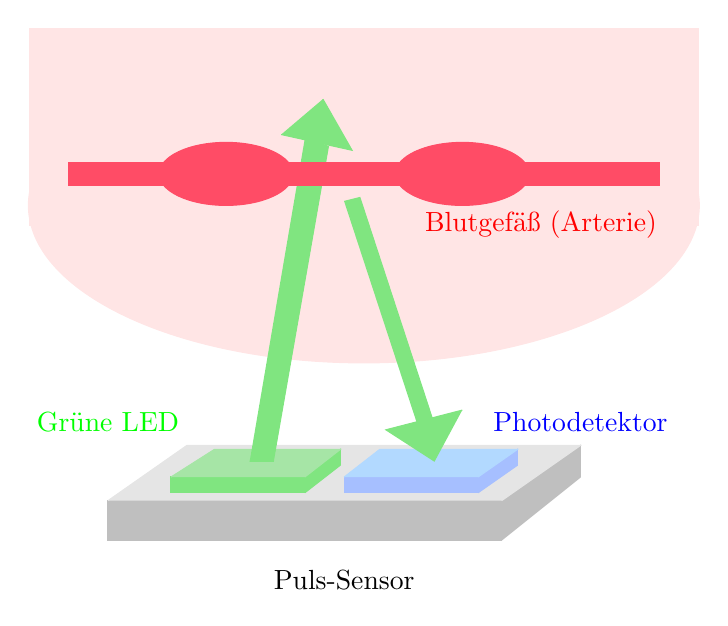
\begin{tikzpicture}
    \draw [fill=lightgray, draw=lightgray] (-2,0) rectangle (3,0.5);
    \draw [fill=lightgray, draw=lightgray] (3,0)--(4,0.8)--(4,1.2)--(3,0.5);
    \definecolor{verylightgray}{gray}{0.9};
    \draw [fill=verylightgray, draw=verylightgray] (-2,0.5)--(-1,1.2)--(4,1.2)--(3,0.5);
    
    \definecolor{lightgreen}{rgb}{0.5, 0.9, 0.5};
    \draw [fill=lightgreen, draw=lightgreen] (-1.2,0.6) rectangle (0.5,0.8);
    \draw [fill=lightgreen, draw=lightgreen] (0.5,0.8)--(0.95,1.15)--(0.95,0.95)--(0.5,0.6);
    
    \definecolor{hautfarbe}{rgb}{1, 0.9, 0.9};
    \draw [fill=hautfarbe, draw=hautfarbe] (-3,4) rectangle (5.5,6.5);
    \draw [fill=hautfarbe, draw=hautfarbe] (1.25,4.25) ellipse (4.26cm and 2cm);
    
    \definecolor{verylightgreen}{rgb}{0.65, 0.9, 0.65};
    \draw [fill=verylightgreen, draw=verylightgreen] (-1.2,0.8)--(-0.65,1.15)--(0.95,1.15)--(0.5,0.8);
    
    \definecolor{lightblue}{rgb}{0.65, 0.75, 1};
    \draw [fill=lightblue, draw=lightblue] (1,0.6) rectangle (2.7,0.8);
    \draw [fill=lightblue, draw=lightblue] (2.7,0.8)--(3.2,1.15)--(3.2,0.95)--(2.7,0.6);
    
    \definecolor{verylightblue}{rgb}{0.7, 0.85, 1};
    \draw [fill=verylightblue, draw=verylightblue] (1,0.8)--(1.45,1.15)--(3.2,1.15)--(2.7,0.8);
    
    \draw [fill=lightgreen, draw=lightgreen] (-0.2,1)--(0.1,1)--(0.8,5)--(0.5,5.1);
    \draw [fill=lightgreen, draw=lightgreen] (0.2,5.15)--(1.1,4.95)--(0.73,5.6);
    \draw [fill=lightgreen, draw=lightgreen] (1,4.3)--(1.2,4.35)--(2.2,1.3)--(2,1.25);
    \draw [fill=lightgreen, draw=lightgreen] (2.15,1)--(1.53,1.4)--(2.5,1.65);
    
    \definecolor{lightred}{rgb}{1, 0.3, 0.4};
    \draw [fill=lightred, draw=lightred] (0,4.5) rectangle (2,4.8);
    \draw [fill=lightred, draw=lightred](-0.5,4.65) ellipse (0.85cm and 0.4cm);
    \draw [fill=lightred, draw=lightred](2.5,4.65) ellipse (0.85cm and 0.4cm);
    \draw [fill=lightred, draw=lightred] (3,4.5) rectangle (5,4.8);
    \draw [fill=lightred, draw=lightred] (-0.5,4.5) rectangle (-2.5,4.8);
    
    \node[green] at (-2,1.5){Grüne LED};
    \node[blue] at (4,1.5){Photodetektor};
    \node at (1,-0.5){Puls-Sensor};
    \node[red] at (3.5,4){Blutgefäß (Arterie)};	
    
  \end{tikzpicture}

        \caption{Photoplethysmographie}
        \label{fig:Photoplethysmographie}	
    \end{figure}
    
    \begin{itemize}
        \item \textbf{Lichtquelle und Fotodetektor:} Der Sensor besteht aus \ac{led}s (meist grünes Licht) und einem Fotodetektor. Die LEDs senden Licht in die Haut.
        \item \textbf{Messung der Lichtreflexion:} Das Licht durchdringt die Haut und wird von den Blutgefäßen reflektiert. Der Fotodetektor misst die Menge des reflektierten Lichts.
        \item \textbf{Erkennung von Blutflussänderungen:} Bei jedem Herzschlag ändert sich die Menge des reflektierten Lichts aufgrund des veränderten Blutflusses in den Blutgefäßen. Diese Änderungen werden vom Fotodetektor erfasst.
        \item \textbf{Berechnung der Herzfrequenz:} Die Änderungen in der Lichtreflexion, die durch den Puls verursacht werden, werden zur Berechnung der Herzfrequenz genutzt.
    \end{itemize}
    
    \subsection{Der Photodetektor}
    
    \begin{itemize}[label={}]
        \item Der Photodetektor nutzt den Photoeffekt, auch als photoelektrischer Effekt bekannt. Der Photoeffekt ist ein physikalisches Phänomen, bei dem Elektronen aus einem Material (meist einem Metall) freigesetzt werden, wenn es mit Licht bestrahlt wird \cite{Traenkler:2014}.
        
        
        \begin{figure}[h]
            \centering
	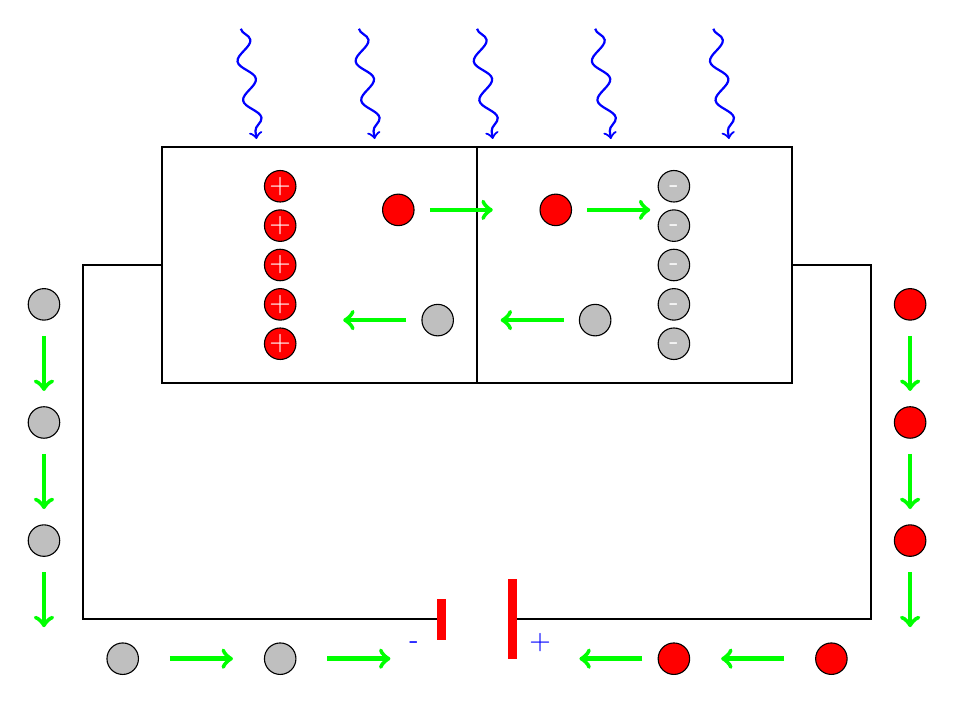
\begin{tikzpicture}
    \draw [thick] (0,0)rectangle(8,3);
    \draw (4,3)--(4,0);
    \draw [thick] (0,1.5)--(-1,1.5)--(-1,-3)--(3.5,-3);
    \draw [thick] (8,1.5)--(9,1.5)--(9,-3)--(4.5,-3);
    \draw [fill=red, draw=red] (3.5,-3.25) rectangle (3.6,-2.75);
    \draw [fill=red, draw=red] (4.5,-3.5) rectangle (4.4,-2.5);
    \node [thick,blue] at(3.2,-3.3){-};
    \node [thick,blue] at(4.8,-3.3){+};
    
    \draw[fill=lightgray] (6.5,0.5) circle (0.2cm);
    \draw[fill=lightgray] (6.5,1) circle (0.2cm);
    \draw[fill=lightgray] (6.5,1.5) circle (0.2cm);
    \draw[fill=lightgray] (6.5,2) circle (0.2cm);
    \draw[fill=lightgray] (6.5,2.5) circle (0.2cm);
    
    \draw[fill=red] (1.5,0.5) circle (0.2cm);
    \draw[fill=red] (1.5,1) circle (0.2cm);
    \draw[fill=red] (1.5,1.5) circle (0.2cm);
    \draw[fill=red] (1.5,2) circle (0.2cm);
    \draw[fill=red] (1.5,2.5) circle (0.2cm);
    
    \draw[fill=lightgray] (5.5,0.8) circle (0.2cm);
    \draw[fill=lightgray] (3.5,0.8) circle (0.2cm);
    
    \draw[->,ultra thick,green](5.1,0.8) -- (4.3,0.8);
    \draw[->,ultra thick,green](3.1,0.8) -- (2.3,0.8);
    
    \draw[fill=red] (3,2.2) circle (0.2cm);
    \draw[fill=red] (5,2.2) circle (0.2cm);
    
    \draw[->,ultra thick,green](3.4,2.2) -- (4.2,2.2);
    \draw[->,ultra thick,green](5.4,2.2) -- (6.2,2.2);
    
    \draw[fill=lightgray] (-1.5,-2) circle (0.2cm);
    \draw[fill=lightgray] (-1.5,1) circle (0.2cm);
    \draw[fill=lightgray] (-1.5,-0.5) circle (0.2cm);
    \draw[fill=lightgray] (-0.5,-3.5) circle (0.2cm);
    \draw[fill=lightgray] (1.5,-3.5) circle (0.2cm);
    
    \draw[->,ultra thick,green](-1.5,0.6) -- (-1.5,-0.1);
    \draw[->,ultra thick,green](-1.5,-0.9) -- (-1.5,-1.6);
    \draw[->,ultra thick,green](-1.5,-2.4) -- (-1.5,-3.1);
    \draw[->,ultra thick,green](0.1,-3.5) -- (0.9,-3.5);
    \draw[->,ultra thick,green](2.1,-3.5) -- (2.9,-3.5);
    
    \draw[fill=red] (9.5,-2) circle (0.2cm);
    \draw[fill=red] (9.5,1) circle (0.2cm);
    \draw[fill=red] (9.5,-0.5) circle (0.2cm);
    \draw[fill=red] (8.5,-3.5) circle (0.2cm);
    \draw[fill=red] (6.5,-3.5) circle (0.2cm);
    
    \draw[->,ultra thick,green](9.5,0.6) -- (9.5,-0.1);
    \draw[->,ultra thick,green](9.5,-0.9) -- (9.5,-1.6);
    \draw[->,ultra thick,green](9.5,-2.4) -- (9.5,-3.1);
    \draw[->,ultra thick,green](7.9,-3.5) -- (7.1,-3.5);
    \draw[->,ultra thick,green](6.1,-3.5) -- (5.3,-3.5);
    
    \draw[thick,blue,->, decorate, decoration={snake, amplitude=1mm, segment length=5mm}] (1,4.5) -- (1.2,3.1);
    \draw[thick,blue,->, decorate, decoration={snake, amplitude=1mm, segment length=5mm}] (2.5,4.5) -- (2.7,3.1);
    \draw[thick,blue,->, decorate, decoration={snake, amplitude=1mm, segment length=5mm}] (4,4.5) -- (4.2,3.1);
    \draw[thick,blue,->, decorate, decoration={snake, amplitude=1mm, segment length=5mm}] (5.5,4.5) -- (5.7,3.1);
    \draw[thick,blue,->, decorate, decoration={snake, amplitude=1mm, segment length=5mm}] (7,4.5) -- (7.2,3.1);
    
    \node [thick,white] at (6.5,0.5) {-};
    \node [thick,white] at (6.5,1) {-};
    \node [thick,white] at (6.5,1.5) {-};
    \node [thick,white] at (6.5,2) {-};
    \node [thick,white] at (6.5,2.5) {-};
    
    \node [thick,white] at (1.5,0.5) {+};
    \node [thick,white] at (1.5,1) {+};
    \node [thick,white] at (1.5,1.5) {+};
    \node [thick,white] at (1.5,2) {+};
    \node [thick,white] at (1.5,2.5) {+};
    
\end{tikzpicture}

            \caption{Der Photoeffekt}
            \label{fig:Photoeffekt}	
        \end{figure}
        
        \item \textbf{Ausgabe des Photodetektors}
        
        Der Photodetektor gibt eine Spannung aus, die über die Zeit gemessen wird. Diese Spannung variiert periodisch in Abhängigkeit von der Menge des reflektierten Lichts, das durch die Blutvolumenänderung aufgrund des Herzschlags beeinflusst wird.
        
        Die Spannungsänderung des Photodetektors ist also gleichzusetzen mit der Frequenz unseres Herzschlags \cite{Traenkler:2014}. 
    \end{itemize}
    
    
    \subsection{Spannungsdatenverarbeitung}
    
    Der Sensor ``GRV Heart Rate 3'' gibt analoge Spannungswerte im Bereich von 0 bis 3,3 Volt aus. Diese Spannungen werden vom Arduino über einen Analogeingang erfasst. Der Arduino nutzt seinen integrierten \ac{adc}, um diese analogen Spannungen in digitale Werte umzuwandeln.
    
    Der \ac{adc} des Arduino hat eine Auflösung von 10 Bit, was bedeutet, dass er Spannungen im Bereich von 0 bis 3,3 Volt in 1024 Schritte unterteilt. Somit wird eine Spannung von 0 Volt als digitaler Wert 0 und eine Spannung von 3,3 Volt als digitaler Wert 1023 dargestellt. Zwischen diesen beiden Extremen werden die Spannungswerte proportional in entsprechende digitale Werte umgewandelt.\cite{Parthier:2016}
    
    Diese Umwandlung ermöglicht es dem Arduino, die vom Sensor ausgegebenen analogen Spannungen als leicht verarbeitbare digitale Werte darzustellen. So kann der Arduino präzise Messungen durchführen und die Herzfrequenzdaten weiterverarbeiten. Im Code werden diese digitalen Werte dann verwendet, um die Herzfrequenz zu berechnen, indem die Anzahl der Spitzenwerte in den Spannungsdaten über eine bestimmte Zeitperiode gezählt und in Schläge pro Minute umgewandelt wird.
    
    \bigskip
    
    \begin{figure}[h]
        \hspace*{-2.5cm} % Verschiebt den Inhalt nach links
        \begin{adjustbox}{valign=t}
	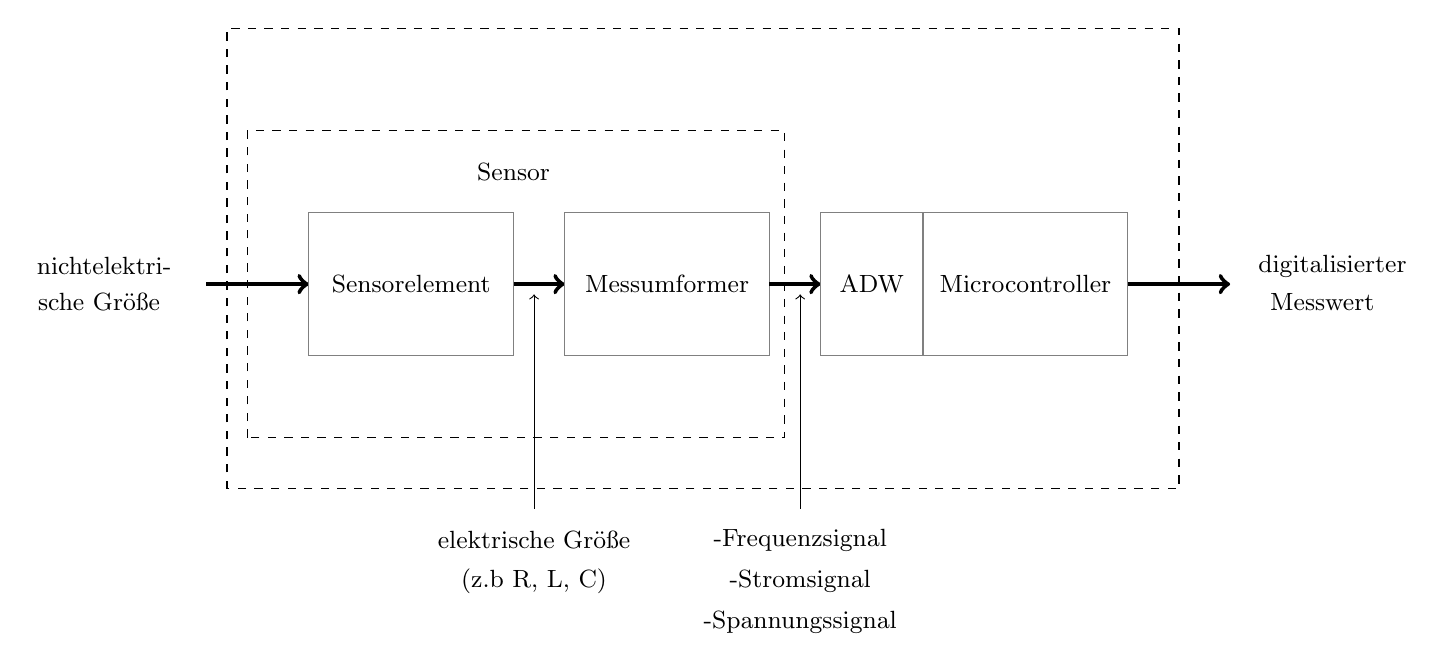
\begin{tikzpicture}[scale=1.3]
    \draw[->,ultra thick](0,0)--(1,0);
    \draw[gray] (1,-0.7) rectangle (3,0.7);
    \draw[->,ultra thick](3,0)--(3.5,0);
    \draw[gray] (3.5,-0.7) rectangle (5.5,0.7);
    \draw[->,ultra thick](5.5,0)--(6,0);
    \draw[gray] (6,-0.7) rectangle (9,0.7);
    \draw[gray] (7,-0.7)--(7,0.7);
    \draw[->,ultra thick](9,0)--(10,0);
    \draw[dashed](0.2,-2)rectangle(9.5,2.5);
    \draw[dashed](0.4,-1.5)rectangle(5.65,1.5);
    
    \draw[<-](3.2,-0.1)--(3.2,-2.2);
    \draw[<-](5.8,-0.1)--(5.8,-2.2);
    
    \node at (3.2,-2.5){\small elektrische Größe};
    \node at (3.2,-2.9){\small (z.b R, L, C)};
    
    \node at (5.8,-2.5){\small -Frequenzsignal};
    \node at (5.8,-2.9){\small -Stromsignal};
    \node at (5.8,-3.3){\small -Spannungssignal};
    
    \node at (3,1.1){\small Sensor};
    \node at (2,0){\small Sensorelement};
    \node at (4.5,0){\small Messumformer};
    \node at (6.5,0){\small ADW};
    \node at (8,0){\small Microcontroller};
    \node at (-1,0.175){\small nichtelektri-};
    \node at (-1.05,-0.175){\small sche Größe};
    
    \node at (11,0.175){\small digitalisierter};
    \node at (10.9,-0.175){\small Messwert};
\end{tikzpicture}

        \end{adjustbox}
        \centering
        \caption{Struktur eines Sensors}
        \label{fig}
    \end{figure}
    
    
    \subsection{Drift und Messungenauigkeiten}
    
    Drift kann eine wichtige Rolle beim Herzschlagsensor spielen. Drift bezieht sich auf die allmähliche Veränderung der Messwerte eines Sensors über die Zeit, die nicht auf tatsächliche Veränderungen des gemessenen Parameters zurückzuführen ist. Im Kontext eines Herzschlagsensors können verschiedene Arten von Drift auftreten.
    
    Ein Herzschlagsensor wandelt physiologische Messgrößen, wie die Blutflussänderungen, in elektrische Signale um, damit diese ausgewertet werden können. Allerdings kann es vorkommen, dass die Messwerte variieren, obwohl die Herzfrequenz konstant bleibt. Diese unerwünschte Veränderung der Messwerte wird als Drift bezeichnet \cite{Traenkler:2014}. Drift ist zeitabhängig und tritt aufgrund von Alterungsprozessen und inhärenten Ungenauigkeiten des Sensors auf. Im schlimmsten Fall kann Drift zu einem funktionalen Ausfall des Sensors führen.
    
    \begin{itemize}[label={}]
        \item  \textbf{Elektronische Drift} bezieht sich auf Veränderungen in der Elektronik des Sensors oder des Arduino-Boards selbst. Elektronische Komponenten können aufgrund von Temperaturänderungen, Alterung oder anderen Faktoren im Laufe der Zeit ihre Eigenschaften verändern, was zu einer Drift der Ausgangswerte führt.
        \item  \textbf{Optische Drift} tritt bei Herzschlagsensoren auf, die auf der Basis von Photoplethysmographie (PPG) arbeiten, indem sie die Lichtabsorption durch das Blut messen. Änderungen in den optischen Komponenten, wie LEDs oder Photodetektoren, können zu Drift führen, beispielsweise durch Verschmutzungen, Alterung der \ac{led}s oder Änderungen in der Durchlässigkeit des Gewebes.
        \item  \textbf{Mechanische Drift} kann durch mechanische Veränderungen oder Verschiebungen des Sensors auf der Haut verursacht werden. Eine schlechte oder sich ändernde Platzierung des Sensors kann die Genauigkeit der Messungen beeinträchtigen.
        \item  \textbf{Kalibrierungsdrift} tritt bei Herzschlagsensoren auf, die regelmäßige Kalibrierungen erfordern, um genaue Messungen zu gewährleisten. Ohne regelmäßige Kalibrierung kann der Sensor anfangen zu driften und ungenaue Messwerte liefern.
    \end{itemize}

    Um die Auswirkungen der Drift zu minimieren, können mehrere Maßnahmen ergriffen werden:
    
    \begin{itemize}[label={}]
        \item \textbf{Regelmäßige Kalibrierung}: Falls der Sensor eine Kalibrierung benötigt, sollte diese regelmäßig durchgeführt werden, um sicherzustellen, dass die Messungen genau bleiben.
        \item \textbf{Kontinuierliche Überwachung}: Durch kontinuierliche Überwachung der Ausgangswerte und Vergleich mit bekannten Referenzwerten (z.B. Vergleich mit einem klinisch validierten Gerät) kann Drift erkannt und korrigiert werden.
        \item \textbf{Platzierung des Sensors}: Eine konsistente und stabile Platzierung des Sensors am Körper kann mechanische Drift minimieren. Idealerweise sollte der Sensor an einer Stelle befestigt werden, die wenig Bewegung ausgesetzt ist, wie das Ohrläppchen.
        \item \textbf{Umgebungskontrolle}: Durch Kontrolle der Umgebungstemperatur und -bedingungen kann elektronische Drift reduziert werden.
    \end{itemize}
    
    Durch die Berücksichtigung dieser Maßnahmen kann die Genauigkeit und Zuverlässigkeit der Herzfrequenzmessungen mit dem Herzschlagsensor verbessert werden \cite{Traenkler:2014}.
    
}


\section{Herzschlagsensor mit Grove-Schnittstelle und Ohr-Clip}

Das Kit ``GRV HEART RATE3 Ear Clip'' besteht aus einem Ohrclip und einem Empfängermodul und ist speziell für die Messung der Herzfrequenz bei Patienten und Sportlern konzipiert. Die gemessenen Daten können entweder in Echtzeit auf einem Monitor über einen seriellen Port angezeigt oder für spätere Analysen gespeichert werden. Das System zeichnet sich durch seine hohe Empfindlichkeit, geringen Stromverbrauch und hohe Mobilität aus. \Mynote{werbung}

\begin{figure}[h]
    \begin{center}
        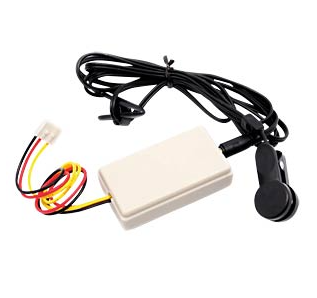
\includegraphics[width=12cm]{HeartRate/HeartRateSensor}
        \caption{Grove-Herzschlag-Sensor mit Ohr-Clip\cite{Seeed:2015}}
        \label{fig:Herzschlagsensor}
    \end{center}
\end{figure}


\subsubsection{Technische Merkmale}

\begin{description}
    \item{Niedriger Stromverbrauch}
    \item{Große Bandbreite beim Eingangsstrom:} 3 - 5 V (Gleichstrom)
    \item{Bequeme Verwendung}
    \item{Hohe Empfindlichkeit}
\end{description}

\subsubsection{Technische Daten}

\begin{description}
    \item{Anschlusstyp:} Steckverbinder JST-VH
    \item{Anschlusssystem:} Grove-Schnittstelle
\end{description} 
\cite{Seeed:2015}



\subsection{Testen des Herzschlagsensors}

Um den Herzschlagsensor zu testen, wird ein einfaches Programm verwendet, mit dem man die Peaks erkennt. Der Herzfrequenzsensor wird an den analogen Pin A0 angeschlossen und der gemessene Wert alle 500 Millisekunden über die serielle Schnittstelle an den Computer gesendet wird. Die serielle Ausgabe über den Plotter wird in einem Diagramm dargestellt, das periodische Herzfrequenzsignale zeigt. Die Werte schwanken zwischen 0 und 1023, was auf die erkannten Peaks des Herzschlagsensors hinweist. Dies bestätigt, dass der Sensor ordnungsgemäß funktioniert und die Herzfrequenzdaten erfolgreich erfasst und visualisiert werden.


\begin{figure}[h]
    \begin{center}
        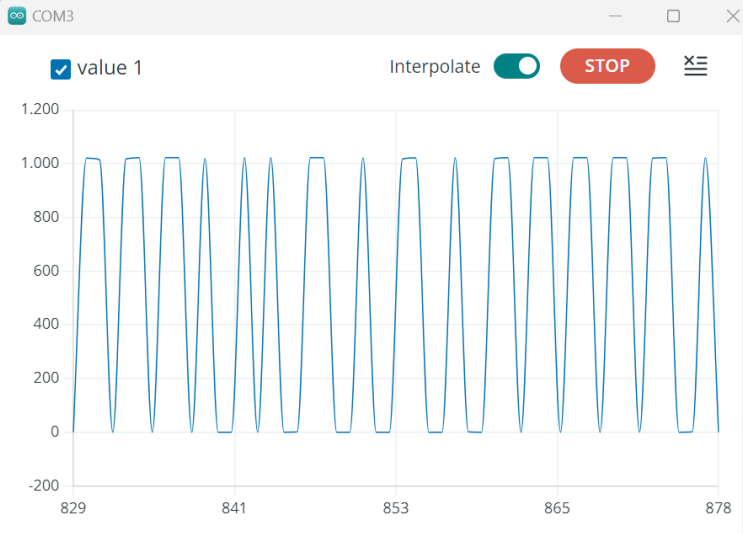
\includegraphics[width=10cm]{HeartRate/HeartRateTestDiagramm}
        \caption{Herzschlag Diagramm (Test)}
        \label{fig:HerzschlagDiagramm}	
    \end{center}
\end{figure}

\begin{code}[h]
    \pythonexternal[language=c++]{../../Code/Arduino/HeartRate/TestHeartRateSensor.ino}
    \caption{Testprogramm Herzschlagsensor} 
    \label{Code:Arduino:HeartRateSensor}
\end{code}


\subsection{Programmcode und Dokumentation}
% Code block with proper placement

\begin{code}[h]
    \
    external[language=c++, linerange={1-11}, firstnumber=1]{../../Code/Arduino/HeartRate/HeartRate.ino}
\end{code}

Zu Beginn des Codes werden die notwendigen Bibliotheken eingebunden. \FILE{Arduino.h} wird für die allgemeine Programmierung auf der Arduino-Plattform benötigt. \FILE{U8g2lib} ist eine Bibliothek für die Ansteuerung von \ac{oled}-Displays, \FILE{SPI.h} und \FILE{SD.h} ermöglichen die Kommunikation mit der SD-Karte. Zusätzlich wird durch bedingte Kompilierung (\PYTHON{\#ifdef U8X8\_HAVE\_HW\_SPI} und \PYTHON{\#ifdef U8X8\_HAVE\_HW\_I2C}) geprüft, ob die Hardware-Schnittstellen \ac{spi} und \ac{i2c} verfügbar sind und die entsprechenden Bibliotheken werden eingebunden, falls sie vorhanden sind. Diese bedingten Einbindungen sind wichtig, um sicherzustellen, dass die richtigen Bibliotheken nur dann geladen werden, wenn die entsprechende Hardware tatsächlich vorhanden ist.

\begin{code}[h]
    \pythonexternal[language=c++, linerange={12-18}, firstnumber=12]{../../Code/Arduino/HeartRate/HeartRate.ino}
\end{code}

In diesen Zeilen wird das Display initialisiert. \PYTHON{U8G2\_SH1106\_128X64\_NONAME\_F\_HW\_I2C u8g2(U8G2\_R0, U8X8\_PIN\_NONE, A5, A4);} erstellt ein Objekt \PYTHON{u8g2} für das OLED-Display, das über \ac{i2c} kommuniziert. Die Pins für den Herzfrequenzsensor (\PYTHON{heartRatePin}), die Batterie (\PYTHON{batteryPin}) und das \ac{sd}-Karten Modul(\PYTHON{chipSelect}) werden ebenfalls definiert.



\begin{code}[h]
    \pythonexternal[language=c++, linerange={19-31}, firstnumber=19]{../../Code/Arduino/HeartRate/HeartRate.ino}
\end{code}

Hier werden verschiedene Variablen definiert, die zur Speicherung und Verarbeitung der Herzfrequenzdaten verwendet werden. \PYTHON{heartRateValue} und \PYTHON{lastHeartRateValue} speichern die aktuellen und vorherigen Herzfrequenzwerte. \PYTHON{lastPeakTime} und \PYTHON{lastHeartbeatTime} speichern die Zeitpunkte der letzten Peaks und Herzschläge. \PYTHON{peakDetected} ist ein boolescher Wert, der angibt, ob ein Peak erkannt wurde. \PYTHON{threshold} ist der Schwellenwert zur Erkennung eines Herzschlags. \PYTHON{heartRate}, \PYTHON{heartRateArray}, \PYTHON{heartRateIndex}, \PYTHON{heartRateSum} und \PYTHON{previousHeartRate} werden zur Berechnung und Speicherung der Herzfrequenz verwendet. \PYTHON{errorTimeout} und \PYTHON{errorState} dienen zur Fehlerüberwachung.


\begin{code}[h]
    \pythonexternal[language=c++, linerange={32-41}, firstnumber=31]{../../Code/Arduino/HeartRate/HeartRate.ino}
\end{code}

\noindent Dieser Abschnitt definiert weitere Variablen zur Steuerung des Anzeigemodus und zur Speicherung der Graphdaten. \PYTHON{lastSwitchTime} und \PYTHON{switchInterval} werden zur Verwaltung des Anzeigemodus verwendet, \PYTHON{showGraph} gibt an, ob der Graph angezeigt wird. \PYTHON{graphData} speichert die Herzfrequenzdaten für die Darstellung im Graphen. \PYTHON{sdCardFull} überprüft, ob die \ac{sd}-Karte voll ist, \PYTHON{startTime} speichert die Startzeit des Arduino und \PYTHON{initialMeasurement} ist ein boolescher Wert, der anzeigt, ob sich das Programm in der initialen Messperiode befindet.



\begin{code}[h]
    \pythonexternal[language=c++, linerange={42-76}, firstnumber=42]{../../Code/Arduino/HeartRate/HeartRate.ino}
\end{code}

Die Funktion  \PYTHON{setup()} initialisiert die serielle Kommunikation mit einer Baudrate von 9600, setzt die Pins für den Herzfrequenzsensor und die Batterie als Eingänge und initialisiert das Display. Zudem wird die \ac{sd}-Karte initialisiert und,  falls die Initialisierung fehlschlägt, wird dies über die serielle Schnittstelle ausgegeben. Anschließend wird ein Startbildschirm auf dem Display angezeigt und die Startzeit gespeichert.

\begin{code}[h]
    \pythonexternal[language=c++, linerange={77-135}, firstnumber=77]{../../Code/Arduino/HeartRate/HeartRate.ino}
\end{code}


\begin{code}[h]
    \pythonexternal[language=c++, linerange={135-173}, firstnumber=135]{../../Code/Arduino/HeartRate/HeartRate.ino}
\end{code}


In der Funktion \PYTHON{loop()} wird die Hauptlogik des Programms ausgeführt. Zunächst wird eine initiale Wartezeit von 5 Sekunden implementiert, um sicherzustellen, dass das System stabil ist, bevor Messungen durchgeführt werden. Falls die \ac{sd}-Karte voll ist, wird die Schleife beendet. Es werden die Herzfrequenz- und Batteriespannungswerte gelesen und die Spannung auf dem seriellen Monitor ausgegeben. Wird ein Herzfrequenzpeak erkannt, wird die Zeit seit dem letzten Peak berechnet und die Herzfrequenz daraus abgeleitet. Diese Werte werden dann auf dem Display angezeigt und auf der \ac{sd}-Karte gespeichert. Zusätzlich werden Graphdaten aktualisiert und Fehlerzustände überwacht. Die Anzeige wechselt alle 10 Sekunden zwischen Text- und Graphmodus, sofern kein Fehlerzustand vorliegt.

\begin{code}[h]
    \pythonexternal[language=c++, linerange={173-183}, firstnumber=173]{../../Code/Arduino/HeartRate/HeartRate.ino}
\end{code}

Die Funktion \PYTHON{drawBattery(float voltage)} zeichnet die Batteriestandsanzeige auf das Display, basierend auf der gemessenen Spannung. Die Spannung wird in einen Wert zwischen 0 und 4 umgewandelt, um den Ladezustand der Batterie darzustellen.


\begin{code}[h]
    \pythonexternal[language=c++, linerange={184-193}, firstnumber=184]{../../Code/Arduino/HeartRate/HeartRate.ino}
\end{code}


In der Funktion \PYTHON{updateGraph(int heartRate)} werden die Herzfrequenzdaten aktualisiert. Die alten Daten werden nach links verschoben und die neue Herzfrequenz wird am Ende des Arrays gespeichert. Falls die Herzfrequenz unter 40 Schläge pro Minute fällt, wird der Wert auf 0 gesetzt. Diese Funktion stellt sicher, dass der Graph immer aktuelle Daten anzeigt und alte Daten kontinuierlich durch neue ersetzt werden.

\begin{code}[h]
    \pythonexternal[language=c++, linerange={195-217}, firstnumber=195]{../../Code/Arduino/HeartRate/HeartRate.ino}
\end{code}

Die Funktion \PYTHON{drawGraph()} zeichnet den Verlauf der Herzfrequenz als Graph auf das Display. Dazu werden die Herzfrequenzdaten über die Zeit aufgetragen und als Liniengraph dargestellt. Die Achsen und Beschriftungen werden ebenfalls gezeichnet. 


\begin{code}[h]
    \pythonexternal[language=c++, linerange={218-237}, firstnumber=218]{../../Code/Arduino/HeartRate/HeartRate.ino}
\end{code}

Die Funktion \PYTHON{saveToSD(int heartRate)} speichert die Herzfrequenzdaten auf der \ac{sd}-Karte. Wenn ein Fehler beim Öffnen der Datei auftritt, wird dies auf dem Display angezeigt und das Programm erkennt, dass die \ac{sd}-Karte voll sein könnte. Dies stellt sicher, dass alle Daten sicher gespeichert werden und der Benutzer informiert wird, falls ein Speicherproblem auftritt.



\section{Kalibrierung}

Wir haben den Herzschlagsensor kalibriert, indem wir die von ihm ausgegebenen Werte gleichzeitig mit den Herzschlagwerten einer Person auf einer Apple Watch abgeglichen und verglichen haben. Erstaunlicherweise stimmten die Werte genau überein, was die Genauigkeit des Sensors bestätigte.

